% !TeX program = lualatex
% !TeX encoding = utf8
% !TeX spellcheck = uk_UA
% !TeX root = ../EMConspect.tex
% УВАГА: для \enquote{...} потрібен пакет csquotes (\usepackage[ukrainian=quotes]{csquotes}
% в преамбулі EMConspect.tex) --- переконайтесь, що він підключений.

%=========================================================
\chapter{Основи електростатики діелектриків}\label{\currfilebase-I}
\graphicspath{{\currfilebase/Pictures}}
%=========================================================
\epigraph{Речовина в електричному полі --- це не пасивне тло, а активний співучасник взаємодії: поле поляризує речовину, а речовина, у відповідь,
	послаблює поле.
}{Переосмислення ідей сучасної фізики}

Цей розділ --- перший із трьох, присвячених електричному полю в діелектриках. Тут ми введемо основні величини ($\vect P$, $\Dfield$, $\epsilon$) і
з'ясуємо, як описувати поле в речовині на макроскопічному рівні. У другому розділі ми побачимо, \emphx{звідки} береться діелектрична проникність
$\epsilon$ і від чого вона залежить на мікроскопічному рівні, а в третьому --- познайомимось із особливими класами діелектриків, чиї властивості
широко використовуються в техніці.

%% --------------------------------------------------------
\section{Основні поняття}
%% --------------------------------------------------------

Досі ми розглядали електричне поле у вакуумі та у провідниках. У провідниках, як ми з'ясували, вільні заряди --- електрони --- під дією як завгодно
слабкого поля переміщуються на макроскопічні відстані, аж доки поле всередині провідника не звернеться в нуль. Проте більшість речовин, що оточують
нас, --- скло, вода, повітря, пластмаси, --- поводяться зовсім інакше: внесені в електричне поле, вони не гасять його всередині себе, а лише
\emphx{послаблюють}. Такі речовини називають \emphx{діелектриками}.

Відмінність діелектрика від провідника пов'язана з тим, які заряди є в його структурі. Домовимось умовно розділяти всі заряди речовини на два типи.

\begin{enumerate}
	\item \emphx{Вільні заряди} --- це заряди, які можуть переміщатися на великі відстані в речовині (набагато більші за міжатомні відстані). Саме
	      вільні заряди відповідають за струм і за повну компенсацію зовнішнього поля всередині провідника. У діелектриках вільних зарядів, як
	      правило, дуже мало, або немає зовсім.
	\item \emphx{Зв'язані (поляризаційні) заряди} --- це заряди, які під дією зовнішніх полів або сил лише незначно \emphx{зміщуються} відносно
	      свого положення рівноваги (електрон у атомі, іон у вузлі кристалічної ґратки) і повертаються назад, у положення рівноваги, одразу після
	      зняття зовнішнього впливу.
\end{enumerate}

\begin{Attention}
	\emphx{Діелектриками} називають речовини, в структурі яких є зв'язані заряди, а вільних зарядів дуже мало або зовсім немає. На відміну від
	провідників, у діелектриках немає носіїв заряду, здатних переміщатися по всьому об'єму тіла: усі заряджені частинки --- електрони та ядра ---
	міцно утримуються в межах свого атома чи молекули.
\end{Attention}

\subsection*{Мікроскопічне та макроскопічне поле}

Щоб коректно описати поведінку речовини в полі, потрібно спершу з'ясувати, про яке саме поле йдеться. Якщо подивитись на речовину на атомному
масштабі, електричне поле виявляється надзвичайно нерівномірним: всередині атома чи молекули воно на багато порядків сильніше, ніж у проміжку між
молекулами, і різко змінюється від точки до точки та в часі --- адже електрони рухаються, атоми коливаються. Таке істинне, швидкозмінне поле
називають \emphx{мікрополем} $\Efield_\text{micro}$.

Усі макроскопічні прилади --- вольтметри, зонди, наші вимірювання --- фізично не здатні відстежити настільки швидкі та дрібномасштабні варіації поля.
Те, що вони фіксують, --- це поле, усереднене по деякому \emphx{фізично нескінченно малому} об'єму $\Delta V$: досить малому порівняно з розмірами
тіла, щоб вважатися \enquote{точкою} в макроскопічному сенсі, але водночас достатньо великому, щоб містити величезну кількість атомів і молекул. Таке
\emphx{середнє (макроскопічне) поле} визначається як
\begin{equation}\label{eq:AvgField}
	\tcbhighmath{
		\left\langle \Efield\right\rangle = \frac1{\Delta V} \iiint\limits_{\Delta V} \Efield_\text{micro}\, dV.
	}
\end{equation}

Це поле змінюється в просторі істотно повільніше, ніж мікрополе, і саме його ми надалі й називатимемо просто $\Efield$, коли говоритимемо про поле
всередині речовини.

%% --------------------------------------------------------
\section{Структура діелектриків}
%% --------------------------------------------------------

\subsection*{Дипольні моменти молекул}

За відсутності зовнішнього поля позитивний заряд ядер атомів, що утворюють молекулу, і негативний заряд електронної оболонки в сумі дають нуль, тобто
молекула електронейтральна. Проте розподіл цих зарядів у просторі не завжди симетричний. Якщо \enquote{центр ваги} позитивного заряду молекули не збігається
з \enquote{центром ваги} негативного, молекула має власний, сталий \emphx{дипольний момент} $\vect p_0$. Причиною такої асиметрії є \emphx{різна
	електронегативність} атомів, що входять до складу молекули: атом з більшою електронегативністю сильніше \enquote{притягує} до себе спільну електронну
хмару, і на ньому виникає надлишок негативного заряду, тоді як на іншому атомі --- надлишок позитивного.

Молекули з ненульовим власним дипольним моментом називають \emphx{полярними}. Класичний приклад --- молекула води $\ce{H2O}$: через кутову форму
молекули (кут між зв'язками O--H становить приблизно $105^\circ$) дипольні моменти окремих зв'язків O--H не компенсують одне одного, і молекула в
цілому має досить великий дипольний момент (рис.~\ref{pic:MoleculeDipoles}).

\begin{figure}[h!]\centering
	\localinput{moleculedipole.tikz}
	\caption{Власні дипольні моменти молекул $\ce{H2O}$ та $\ce{NH3}$\label{pic:MoleculeDipoles}}
\end{figure}

Для вимірювання дипольних моментів молекул зручно користуватись позасистемною одиницею --- \emphx{дебаєм} (позначається \textit{Д} або \textit{D}),
названою на честь фізика П.~Дебая:
\begin{equation*}
	1\ \text{Дебай} = 10^{-18}\ \text{Фр}\cdot\text{см}.
\end{equation*}
Більшість полярних молекул має дипольний момент порядку $1$ Д. Одиниця широко застосовується у фізичній хімії, атомній і молекулярній фізиці.
Дипольні моменти деяких відомих полярних молекул наведено в таблиці~\ref{tab:dipoles}.

\begin{table}[h!]
	\centering
	\caption{Дипольні моменти деяких полярних молекул\label{tab:dipoles}}
	\begin{tabular}{lc}
		\toprule
		Молекула                    & Дипольний момент (Дебай) \\
		\midrule
		Вода ($\ce{H2O}$)           & 1.84                      \\
		Аміак ($\ce{NH3}$)          & 1.46                      \\
		Вуглекислий газ ($\ce{CO2}$) & 0.00                     \\
		Хлороводень ($\ce{HCl}$)    & 1.08                      \\
		Метанол ($\ce{CH3OH}$)      & 1.70                      \\
		\bottomrule
	\end{tabular}
\end{table}

Показовим є приклад вуглекислого газу $\ce{CO2}$: незважаючи на те, що кожен зв'язок C=O є полярним, молекула лінійна і симетрична, тому дипольні
моменти окремих зв'язків повністю компенсують одне одного, і сумарний дипольний момент молекули дорівнює нулю.

\subsection*{Неполярні молекули та наведений дипольний момент}

\emphx{Неполярні молекули} --- це молекули, в яких електричні заряди розподілені симетрично, і власний дипольний момент відсутній ($p_0 = 0$).
У таких молекулах атоми зазвичай мають однакову або близьку електронегативність, тому спільна електронна хмара розподілена рівномірно між
атомами, або ж молекула має достатньо високу симетрію (як у випадку $\ce{CO2}$). Прикладами неполярних молекул є кисень $\ce{O2}$, азот
$\ce{N2}$, метан $\ce{CH4}$, а також окремі атоми інертних газів.

Важливо розуміти, що відсутність \emphx{власного} дипольного моменту не означає, що неполярна молекула взагалі не може мати дипольного моменту. У
зовнішньому електричному полі позитивно заряджене ядро і негативно заряджена електронна хмара зміщуються в протилежні боки: ядро --- за полем,
електрони --- проти поля (рис.~\ref{pic:InducedDipole}). В результаті \enquote{центри ваги} позитивного та негативного зарядів розходяться, і в молекулі
виникає \emphx{наведений (індукований) дипольний момент}, пропорційний прикладеному полю:
\begin{equation}\label{eq:InducedDipole}
	\vect p = \alpha \Efield,
\end{equation}
де коефіцієнт $\alpha$ називають \emphx{поляризовністю молекули}.

\begin{figure}[h!]\centering
	\localinput{nonpolar-molecule.tikz}
	\caption{Неполярна молекула без зовнішнього поля та в зовнішньому полі\label{pic:InducedDipole}}
\end{figure}

Цей механізм появи дипольного моменту називають \emphx{електронною (деформаційною) поляризацією}: оскільки маса електронної хмари набагато менша за
масу ядра, саме зміщення електронної хмари відносно ядра і дає основний внесок у наведений момент. На відміну від орієнтаційного механізму, який ми
розглянемо в п.~\ref{sec:Langevin-Debye}, електронна поляризовність практично не залежить від температури.

%% --------------------------------------------------------
\section{Поляризація діелектриків}
%% --------------------------------------------------------

\begin{Attention}
	\emphx{Поляризація} --- це просторовий \emphx{перерозподіл зв'язаних зарядів}, що призводить до виникнення об'ємного дипольного моменту
	середовища. Поляризація може виникати як під дією зовнішнього електричного поля, так і під впливом інших зовнішніх чинників --- механічної
	деформації, зміни температури тощо.
\end{Attention}

Розглянемо, як відбувається поляризація в двох основних класах діелектриків.

\begin{itemize}
	\item \emphx{Полярні діелектрики} складаються з полярних молекул, кожна з яких уже має власний дипольний момент $\vect p_0 \neq 0$. За
	      відсутності зовнішнього поля теплове (хаотичне) обертання молекул орієнтує їхні дипольні моменти цілком випадково в усіх напрямках, тому в
	      будь-якому фізично малому об'ємі дипольні моменти в середньому взаємно компенсуються, і сумарний дипольний момент речовини дорівнює нулю.
	      Коли ж прикладене зовнішнє поле, воно створює момент сил, що прагне розвернути кожен диполь уздовж поля (див.~формулу
	      $\vect M = [\vect p\times\Efield]$, отриману в попередньому розділі). Тепловий рух заважає ідеальному впорядкуванню, проте певна переважна
	      орієнтація вздовж поля все ж встановлюється --- виникає так звана \emphx{орієнтаційна поляризація}.
	\item \emphx{Неполярні діелектрики} складаються з неполярних молекул, у яких за відсутності поля центри позитивного й негативного зарядів
	      збігаються. Зовнішнє поле зміщує електронні хмари відносно ядер (формула~\eqref{eq:InducedDipole}), і в кожній молекулі виникає наведений
	      дипольний момент, зорієнтований уздовж поля, --- \emphx{електронна поляризація}.
\end{itemize}

% ==================== FIGURE 1: полярні молекули ====================
\begin{figure}[h!]
	\centering
	% --- (а) кадр 1: полярні молекули без поля ---
	\begin{subfigure}[t]{0.48\linewidth}
		\centering
		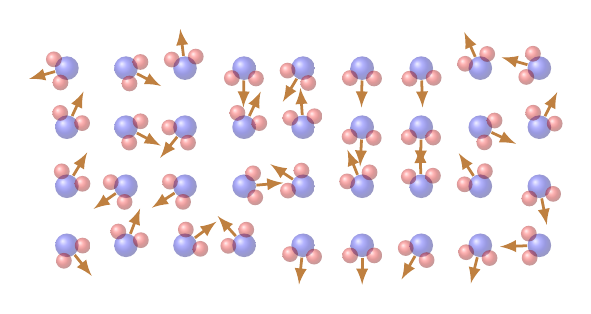
\begin{tikzpicture}[>=latex]
			\pgfmathsetseed{1}
			\tikzset{
				water/.pic={
						\begin{scope}[opacity=0.4]
							\node[circle, ball color=blue, inner sep=0, minimum size=0.3cm] (O) at
							(0,0) {};
							\node[circle, ball color=red, inner sep=0, minimum size=0.2cm] (H1) at
							(-50:0.2) {};
							\node[circle, ball color=red, inner sep=0, minimum size=0.2cm] (H2) at
							(50:0.2) {};
						\end{scope}
						\draw[-latex, brown, line width=1pt] (O) -- ++(0.5, 0);
					},
			}
			\foreach \x in {0,...,8}
				{
					\foreach \y in {0,...,3}{
							\pic[rotate={random(0,360)}] at ({0.75*\x}, {0.75*\y}) {water};
						}
				}
		\end{tikzpicture}
		\caption{Без поля}
		\label{pic:PolarNoField}
	\end{subfigure}\hfill
	% --- (б) кадр 2: полярні молекули в полі ---
	\begin{subfigure}[t]{0.48\linewidth}
		\centering
		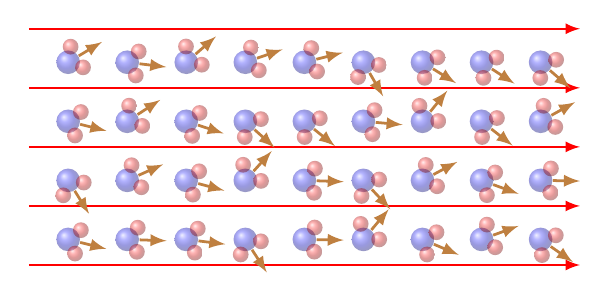
\begin{tikzpicture}[>=latex]
			\pgfmathsetseed{1}
			\tikzset{
				water/.pic={
						\begin{scope}[opacity=0.4]
							\node[circle, ball color=blue, inner sep=0, minimum size=0.3cm] (O) at
							(0,0) {};
							\node[circle, ball color=red, inner sep=0, minimum size=0.2cm] (H1) at
							(-50:0.2) {};
							\node[circle, ball color=red, inner sep=0, minimum size=0.2cm] (H2) at
							(50:0.2) {};
						\end{scope}
						\draw[-latex, brown, line width=1pt] (O) -- ++(0.5, 0);
					},
			}
			\foreach \y in {0,...,4} {
					\draw[->, red, thick] (-0.5,{0.75*\y-0.325}) -- ++(7,0);
				}
			\foreach \x in {0,...,8}
				{
					\foreach \y in {0,...,3}{
							\pic[rotate={random(-60,60)}] at ({0.75*\x}, {0.75*\y}) {water};
						}
				}
		\end{tikzpicture}
		\caption{У полі}
		\label{pic:PolarField}
	\end{subfigure}
	\caption{Поляризація полярних молекул: у зовнішньому електричному полі
		диполі орієнтуються вздовж поля}
	\label{pic:PolarizationPolar}
\end{figure}

% ==================== FIGURE 2: неполярні молекули ====================
\begin{figure}[h!]
	\centering
	% --- (а) кадр 3: неполярні молекули без поля ---
	\begin{subfigure}[t]{0.48\linewidth}
		\centering
		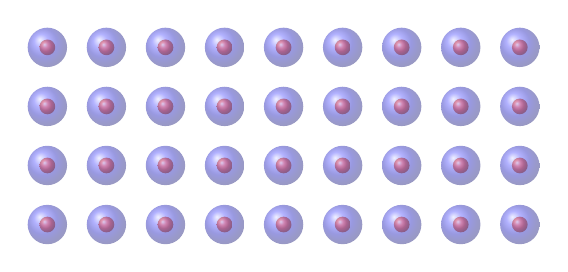
\begin{tikzpicture}[>=latex]
			\tikzset{
				unperturbed/.pic={
						\begin{scope}[opacity=0.4]
							\node[circle, ball color=blue, inner sep=0, minimum size=0.5cm] (O) at
							(0,0) {};
							\node[circle, ball color=red, inner sep=0, minimum size=0.2cm] (H1) at
							(0,0) {};
						\end{scope}
					},
			}
			\foreach \x in {0,...,8}
				{
					\foreach \y in {0,...,3}{
							\pic[] at ({0.75*\x}, {0.75*\y}) {unperturbed};
						}
				}
		\end{tikzpicture}
		\caption{Без поля}
		\label{pic:NonPolarNoField}
	\end{subfigure}\hfill
	% --- (б) кадр 4: неполярні молекули в полі ---
	\begin{subfigure}[t]{0.48\linewidth}
		\centering
		\begin{tikzpicture}[>=latex]
			\tikzset{
				perturbed/.pic={
						\begin{scope}[opacity=0.4]
							\node[ellipse, ball color=blue, inner sep=0, minimum width=0.6cm,
								minimum height=0.4cm] (O) at
							(-0.1,0) {};
							\node[circle, ball color=red, inner sep=0, minimum size=0.2cm] (H1) at
							(+0.02,0) {};
						\end{scope}
						\draw[-latex, brown, line width=1pt] (-0.2,0) -- ++(0.5, 0);
					},
			}
			\foreach \y in {0,...,4} {
					\draw[->, red, thick] (-0.5,{0.75*\y-0.325}) -- ++(7,0);
				}
			\foreach \x in {0,...,8}
				{
					\foreach \y in {0,...,3}{
							\pic[] at ({0.75*\x}, {0.75*\y}) {perturbed};
						}
				}
		\end{tikzpicture}
		\caption{У полі}
		\label{pic:NonPolarField}
	\end{subfigure}
	\caption{Поляризація неполярних молекул: у зовнішньому електричному полі
		молекули деформуються, утворюючи індукований дипольний момент}
	\label{pic:PolarizationNonPolar}
\end{figure}

У випадку йонних кристалів (наприклад, $\ce{NaCl}$) існує ще один механізм --- \emphx{йонна поляризація}: позитивні та негативні йони кристалічної
ґратки під дією поля зміщуються один відносно одного як цілі підґратки, що також створює об'ємний дипольний момент. Детальніше про всі три механізми
(електронний, йонний, орієнтаційний) і про те, як кожен із них залежить від частоти поля й температури, йтиметься в розділі~II
(п.~\ref{sec:AtomPolarizability}).

В обох випадках --- полярних і неполярних діелектриків --- результат один: на межах виділеного в речовині об'єму з'являються надлишкові
(некомпенсовані) зв'язані заряди, тоді як в основному об'ємі речовини позитивні та негативні заряди сусідніх диполів взаємно компенсують одне одного.
Саме ці надлишкові поверхневі заряди і створюють власне поле речовини $\Efield'$, яке, за принципом суперпозиції, додається до зовнішнього поля
$\Efield_\text{ex}$:
\begin{equation*}
	\Efield = \Efield_\text{ex} + \Efield'.
\end{equation*}
Оскільки диполі орієнтуються так, що їхні позитивні полюси \enquote{дивляться} за полем, а негативні --- проти поля, власне поле $\Efield'$ спрямоване
\emphx{назустріч} зовнішньому, і сумарне поле в діелектрику завжди \emphx{послаблюється} порівняно з зовнішнім.

На рисунку~\ref{pic:PolarizedDielectric} схематично показано поляризований
діелектрик у зовнішньому електричному полі: на протилежних поверхнях
виділеного об'єму виникають некомпенсовані зв'язані заряди $-Q$ та $+Q$,
власне поле яких спрямоване назустріч зовнішньому.

\begin{figure}[h!]
	\centering
	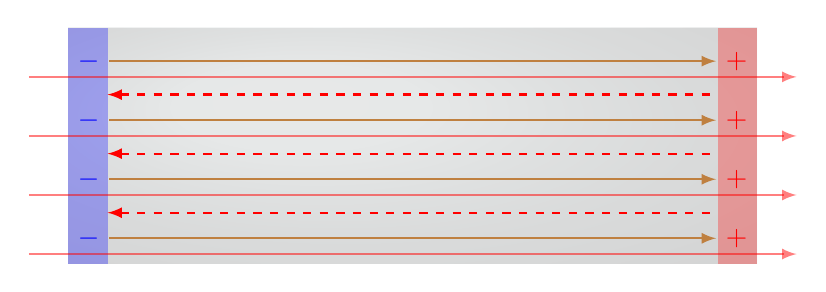
\begin{tikzpicture}[>=latex]
		\begin{scope}
			\fill[ball color=cyan!10, opacity=0.1] (-0.5,{0.75*0-0.325}) rectangle
			++(8.75,{0.75*4});
			\fill[blue, opacity=0.3] (-0.5,{0.75*0-0.325}) rectangle ++(0.5, {0.75*4});
			\fill[red, opacity=0.3] (7.75,{0.75*0-0.325}) rectangle ++(0.5, {0.75*4});
		\end{scope}
		\foreach \y in {0,...,3} {
				\path[] (-0.5,{0.75*\y}) node[right, text=blue] (-Q) {$-$} ++(8.75,0)
				node[left, text=red] (+Q) {$+$};
				\draw[->, brown, thick] (-Q) -- (+Q);

				\ifnum\y<3
					\draw[<-, red, thick, dashed] (0,{0.75*\y+0.325}) -- ++(7.75,0);
				\fi

				\draw[->, red, thick, opacity=0.5] (-1,{0.75*\y-0.2}) -- ++(9.75,0);
			}
	\end{tikzpicture}
    \caption{Поляризований діелектрик у зовнішньому електричному полі:
    	на поверхнях виникають зв'язані заряди $-Q$ та $+Q$. Стрілки означають:
    	\protect\tikz[baseline=-0.6ex]{\protect\draw[->, red, thick, opacity=0.5] (0,0) -- (0.6,0);}
    	--- зовнішнє поле $\Efield_\text{ex}$;
    	\protect\tikz[baseline=-0.6ex]{\protect\draw[<-, red, thick, dashed] (0,0) -- (0.6,0);}
    	--- поле зв'язаних зарядів $\Efield'$;
    	\protect\tikz[baseline=-0.6ex]{\protect\draw[->, brown, thick] (0,0) -- (0.6,0);}
    	--- вектор поляризації $\vect{P}$ (також співпадає з результуючим полем $\Efield$).
    }
	\label{pic:PolarizedDielectric}
\end{figure}

\subsection*{Електрострикція}

Уміщення діелектрика в електричне поле призводить не лише до поляризації, а й до \emphx{зміни розмірів тіла} --- явища, яке називають
\emphx{електрострикцією}. Електрострикція спостерігається в усіх без винятку діелектриках, проте в переважній більшості матеріалів виражена слабко:
деформація пропорційна \emphx{квадрату} поля, $\Delta \ell \sim E^2$, тому не залежить від напрямку поля (зміна знака поля не змінює знака деформації) і
стає помітною лише в дуже сильних полях. У техніці електрострикцію майже завжди \enquote{перекриває} значно сильніший \emphx{п'єзоефект}
(п.~\ref{sec:PiezoPyro}), тому як самостійне явище вона застосовується рідко.

%% --------------------------------------------------------
\section{Вектор поляризації}
%% --------------------------------------------------------

Для кількісного опису стану поляризованого діелектрика вводять \emphx{макроскопічну} характеристику --- \emphx{вектор поляризації} (або
\emphx{поляризованість}), який дорівнює дипольному моменту одиниці об'єму речовини:
\begin{equation}\label{eq:Pdef}
	\tcbhighmath{
		\vect P = \frac1V \sum_i \vect p_i,
	}
\end{equation}
де підсумовування проводиться за всіма молекулярними диполями $\vect p_i$, що потрапляють у фізично малий об'єм $V$.

Для великого класу діелектриків, що не надто відрізняються за своїми властивостями від вакууму (гази, більшість рідин та аморфних твердих тіл за не
надто сильних полів), експериментально встановлено, що поляризованість лінійно залежить від напруженості поля \emphx{в самому діелектрику}:
\begin{equation}\label{eq:PlinearE}
	\tcbhighmath{
		\vect P = \chi \Efield,
	}
\end{equation}
де безрозмірна величина $\chi > 0$ називається \emphx{поляризовністю речовини} (у частині літератури цю ж величину називають \emphx{діелектричною
сприйнятливістю} --- термін цілком рівноправний, проте надалі ми користуватимемось терміном \enquote{поляризовність}, підкреслюючи його спорідненість
з поляризовністю окремої молекули $\alpha$, формула~\eqref{eq:InducedDipole}: перша --- мікроскопічна, друга --- макроскопічна характеристики того
самого явища, а нетривіальний зв'язок між ними --- предмет розділу~II). Поляризовність $\chi$
не залежить від $\Efield$ і характеризує властивості самого діелектрика (тип молекул, їхню концентрацію, температуру тощо). Такі діелектрики
називають \emphx{лінійними}.

\begin{Attention}
	Не всі діелектрики є лінійними. Існують діелектрики, для яких співвідношення $\vect P = \chi\Efield$ не виконується: деякі йонні кристали,
	електрети, а особливо --- сегнетоелектрики, для яких зв'язок між $\vect P$ і $\Efield$ нелінійний і до того ж неоднозначний (див.~розділ~III).
	Докладніше про нелінійні діелектрики, анізотропію та тензор поляризовності йтиметься в розділі~II (п.~\ref{sec:PolTensor}).
\end{Attention}

\subsection*{Однорідна та неоднорідна поляризація}

Поляризацію називають \emphx{однорідною}, якщо вектор $\vect P$ є сталим у всьому об'ємі речовини, $\vect P = \const$, і \emphx{неоднорідною}, якщо
$\vect P$ змінюється від точки до точки.

\emphx{Однорідна поляризація.} Нехай поляризація однорідна. Розглянемо косокутний паралелепіпед, вирізаний із поляризованої речовини так, що його
бічне ребро паралельне вектору поляризації $\vect P$ (рис.~\ref{pic:PolarizedParallelepiped}). Якщо $S$ --- площа бічної грані, а $\ell$ --- довжина
ребра паралелепіпеда, то його об'єм дорівнює $V = S\ell\cos\theta$, де $\theta$ --- кут між ребром $\vect \ell$ і нормаллю до бічної грані.

\begin{figure}[h!]\centering
	\localinput{parallelepiped.tikz}
	\caption{Косокутний паралелепіпед, вирізаний з однорідно поляризованого діелектрика уздовж
		вектора поляризації $\vect P$\label{pic:PolarizedParallelepiped}}
\end{figure}

Диполі всередині такого паралелепіпеда шикуються \enquote{голова до хвоста}: позитивний заряд одного диполя сусідить з негативним зарядом наступного, і в
об'ємі речовини ці заряди взаємно компенсуються. Некомпенсованими лишаються тільки заряди на двох торцевих гранях: на одній виступає надлишковий
позитивний заряд, на іншій --- негативний. Тому весь паралелепіпед еквівалентний одному великому диполю з дипольним моментом $\vect p = \sigma' S
	\vect \ell$, де $\sigma'$ --- поверхнева густина \emphx{зв'язаного (поляризаційного)} заряду на торцевій грані. З іншого боку, за
означенням~\eqref{eq:Pdef}, дипольний момент паралелепіпеда дорівнює $\vect p = \vect P \cdot V = \vect P \, S\ell\cos\theta$. Прирівнюючи обидва
вирази і враховуючи, що $\vect P \cdot \vect n = P\cos\theta$ (де $\vect n$ --- зовнішня нормаль до грані), отримуємо просту й важливу формулу:
\begin{equation}\label{eq:SigmaPrime}
	\tcbhighmath{
		\vect P \cdot \vect n = P_n = \sigma'.
	}
\end{equation}

\begin{Attention}
	Нормальна складова вектора поляризації на поверхні діелектрика чисельно дорівнює поверхневій густині зв'язаного заряду, що виступає на цій
	поверхні. Там, де вектор $\vect P$ спрямований \emphx{із} речовини (нормальна складова додатна), на поверхні виступає позитивний зв'язаний
	заряд; там, де $\vect P$ спрямований \emphx{у} речовину, --- негативний.
\end{Attention}

\emphx{Неоднорідна поляризація.} Нехай тепер поляризація неоднорідна, і в товщі речовини виділено об'єм $V$ довільної форми, обмежений замкненою
поверхнею $S$ (рис.~\ref{pic:NonUniformPolarization}). Кожен малий елемент поверхні $dS$ можна, як і вище, вважати гранню елементарного косокутного
паралелепіпеда, тому на ньому виступає поверхневий зв'язаний заряд $d q' = \sigma' dS = P_n\, dS$.

\begin{figure}[h!]\centering
	\localinput{nonuniform-polarization.tikz}
	\caption{Довільний об'єм неоднорідно поляризованого діелектрика: на поверхні виступають
		некомпенсовані зв'язані заряди\label{pic:NonUniformPolarization}}
\end{figure}

Підсумовуючи (інтегруючи) цей вираз за всією замкненою поверхнею, знаходимо повний
заряд, що вийшов на зовнішню поверхню виділеного об'єму:
\begin{equation*}
	q'_{\text{пов}} = \oiint\limits_S P_n\, dS.
\end{equation*}
Але сама речовина, з якої вирізано цей об'єм, електронейтральна: поляризація лише \emphx{перерозподіляє} наявні заряди, не створюючи нових. Тому
якщо на зовнішню поверхню вийшов заряд $q'_{\text{пов}}$, то всередині об'єму мусив залишитися зв'язаний заряд протилежного знака, розподілений з
об'ємною густиною $\rho'$:
\begin{equation}\label{eq:GaussForP-int}
	\tcbhighmath{
		\oiint\limits_S \vect P\cdot d\vect S = \oiint\limits_S P_n\, dS = - \iiint\limits_V \rho'\, dV.
	}
\end{equation}
Це співвідношення називають \emphx{теоремою Гаусса для вектора поляризації}: воно за формою повністю аналогічне теоремі Гаусса для поля $\Efield$
(п.~\ref{sec:Gauss}), проте зв'язує потік вектора $\vect P$ не з повним, а лише зі \emphx{зв'язаним} зарядом, узятим із протилежним знаком.

Так само, як ми переходили від інтегральної форми теореми Гаусса для $\Efield$ до диференціальної, стягуючи об'єм $V$ у точку, з
формули~\eqref{eq:GaussForP-int} отримуємо \emphx{диференціальну форму теореми Гаусса для вектора поляризації}:
\begin{equation}\label{eq:GaussForP-diff}
	\tcbhighmath{
		\divg \vect P = -\rho'.
	}
\end{equation}
Дивергенція вектора поляризації в даній точці дорівнює об'ємній густині зв'язаного заряду в цій точці, узятій зі знаком мінус. У окремому випадку
однорідної поляризації, коли $\vect P = \const$, маємо $\divg \vect P \equiv 0$, а отже, і $\rho' = 0$: об'ємний зв'язаний заряд в однорідно
поляризованому діелектрику відсутній, увесь надлишковий заряд зосереджений на поверхні, що узгоджується з розглянутим вище прикладом
паралелепіпеда.

%% --------------------------------------------------------
\section{Вектор електричної індукції}\label{sec:Dfield}
%% --------------------------------------------------------

Електричне поле всередині речовини створюється не лише вільними, а й зв'язаними (поляризаційними) зарядами. Тому в теоремі Гаусса для поля
$\Efield$ (яка, нагадаємо, є універсальним законом і виконується для будь-яких зарядів) слід урахувати обидва типи зарядів --- і вільні $\rho$, і
зв'язані $\rho'$:
\begin{equation*}
	\divg \Efield = 4\pi(\rho + \rho').
\end{equation*}
Скориставшись знайденим щойно співвідношенням~\eqref{eq:GaussForP-diff}, а саме $\rho' = -\divg\vect P$, отримуємо:
\begin{equation*}
	\divg \Efield = 4\pi\rho - 4\pi \divg\vect P
	\quad\Longrightarrow\quad
	\divg\left(\Efield + 4\pi \vect P\right) = 4\pi\rho.
\end{equation*}
Вираз у дужках зручно позначити окремим символом і назвати \emphx{вектором електричної індукції}:
\begin{equation}\label{eq:Ddef}
	\tcbhighmath{
		\Dfield = \Efield + 4\pi\vect P.
	}
\end{equation}
Тоді теорема Гаусса для електричного поля \emphx{в речовині} набуває вигляду
\begin{equation}\label{eq:GaussForD-diff}
	\tcbhighmath{
		\divg\Dfield = 4\pi\rho,
	}
\end{equation}
а в інтегральній формі --- відповідно
\begin{equation}\label{eq:GaussForD-int}
	\tcbhighmath{
		\oiint\limits_S \Dfield\cdot d\vect S = 4\pi \iiint\limits_V \rho\, dV.
	}
\end{equation}

\begin{Attention}
	У формулювання теореми Гаусса для поля в речовині входять \emphx{тільки вільні заряди} $\rho$. Внесок зв'язаних (поляризаційних) зарядів уже
	враховано --- він \enquote{захований} усередині означення вектора індукції $\Dfield$. Саме тому вектор $\Dfield$ є надзвичайно зручним інструментом:
	для обчислення його потоку крізь довільну поверхню достатньо знати лише розподіл \emphx{вільних} зарядів, які, на відміну від зв'язаних, як
	правило, відомі заздалегідь (наприклад, задані зарядом на обкладинках конденсатора).
\end{Attention}

Підкреслимо: на відміну від $\Efield$, вектор $\Dfield$ \emphx{не} є потенціальним силовим полем у звичайному розумінні --- він не діє безпосередньо
на пробний заряд. Це допоміжна, суто розрахункова величина, яка водночас має ясний фізичний зміст: вона \enquote{відстежує} тільки ті заряди, якими ми
керуємо ззовні (вільні), незалежно від того, який діелектрик їх оточує.

\subsection*{Діелектрична проникність}

Для лінійних діелектриків, у яких справедливе співвідношення~\eqref{eq:PlinearE}, вектор індукції теж виявляється пропорційним $\Efield$:
\begin{equation*}
	\Dfield = \Efield + 4\pi\vect P = \Efield + 4\pi\chi\Efield = (1+4\pi\chi)\Efield.
\end{equation*}
Позначаючи
\begin{equation}\label{eq:eps}
	\tcbhighmath{
		\epsilon = 1 + 4\pi\chi,
	}
\end{equation}
отримуємо просте й дуже часто використовуване співвідношення
\begin{equation}\label{eq:DepsE}
	\tcbhighmath{
		\Dfield = \epsilon\Efield.
	}
\end{equation}
Величину $\epsilon$ називають \emphx{діелектричною проникністю середовища}. Оскільки для звичайних (не сегнетоелектричних) речовин у постійних полях
завжди $\chi > 0$, то й $\epsilon > 1$: діелектрична проникність будь-якого \enquote{нормального} діелектрика перевищує одиницю. Для вакууму, в якому
поляризація відсутня ($\chi = 0$), маємо $\epsilon = 1$, і вектори $\Dfield$ та $\Efield$ збігаються.

Для орієнтації наведемо порядки величин $\epsilon$ для кількох типових речовин (постійне поле, кімнатна температура):
\begin{center}
	\begin{tabular}{lc@{\qquad}lc}
		\toprule
		Речовина & $\epsilon$ & Речовина & $\epsilon$ \\
		\midrule
		Повітря (сухе) & $1{,}0006$ & Вода & $81$ \\
		Скло & $5$--$7$ & Титанат барію ($\ce{BaTiO3}$) & $10^3$--$10^4$ \\
		\bottomrule
	\end{tabular}
\end{center}
Бачимо, що для газів $\epsilon$ дуже близька до одиниці (молекули далеко одна від одної), для рідин і твердих тіл --- суттєво більша, а для
сегнетоелектриків (розділ~III) сягає аномально великих значень.

\emphx{Приклад.} Розглянемо точковий заряд $Q$, вміщений у нескінченний однорідний діелектрик з проникністю $\epsilon$
(рис.~\ref{pic:PointChargeDielectric}). Через сферичну симетрію
задачі, за теоремою Гаусса для вектора $\Dfield$, як і у випадку поля у вакуумі,
\begin{equation*}
	\Dfield = \frac{Q}{r^2}\frac{\vect r}{r},
\end{equation*}
а звідси, користуючись~\eqref{eq:DepsE}, знаходимо напруженість поля безпосередньо в діелектрику:
\begin{equation*}
	\Efield = \frac{\Dfield}{\epsilon} = \frac{Q}{\epsilon r^2}\frac{\vect r}{r}.
\end{equation*}
Оскільки $\epsilon > 1$, поле точкового заряду в діелектрику всюди \emphx{слабкіше}, ніж таке саме поле у вакуумі. Наприклад, у воді
($\epsilon \approx 81$) поле на тій самій відстані від заряду слабкіше у $81$ раз, а у склі ($\epsilon \approx 5$) --- у $5$ разів. Це прямий
кількісний прояв уже відомого нам якісного результату: \emphx{поляризаційні заряди, що виникають навколо заряду $Q$, послаблюють його поле}.

\begin{figure}[h!]\centering
	\localinput{point-charge-dielectric.tikz}
	\caption{Точковий заряд у нескінченному однорідному діелектрику\label{pic:PointChargeDielectric}}
\end{figure}

%% --------------------------------------------------------
\section{Граничні умови в присутності діелектриків}
%% --------------------------------------------------------

Як і у випадку поля у вакуумі (п.~\ref{sec:BC}), на межі розділу двох середовищ (двох діелектриків, або діелектрика й вакууму) поле може змінюватись
стрибком. Знайдемо, як пов'язані значення полів по обидва боки межі.

\emphx{Перша гранична умова (для нормальної складової $\Dfield$).} Застосуємо теорему Гаусса для вектора $\Dfield$ до нескінченно малого циліндра,
що охоплює невелику ділянку межі розділу середовищ 1 та 2, так само, як ми робили це для поля $\Efield$ на поверхні провідника (рис.~\ref{pic:BC1}).
Нехай $\sigma$ ---
поверхнева густина \emphx{вільного} заряду на межі розділу (якщо він там є). Враховуючи, що $d\vect S_1 = -d\vect S_2 = \vect n\, dS$, де $\vect n$
--- нормаль, спрямована з середовища 1 у середовище 2, маємо

\begin{figure}[h!]\centering
	\localinput{bc1.tikz}
	\caption{Циліндр Гаусса на межі розділу двох середовищ для виведення граничної умови на
		нормальну складову $\Dfield$\label{pic:BC1}}
\end{figure}
\begin{equation*}
	\oiint\limits_S \Dfield\cdot d\vect S = 4\pi\sigma \, dS
	\quad\Longrightarrow\quad
	\Dfield_2 \cdot d\vect S_2 + \Dfield_1\cdot d\vect S_1 \equiv (D_{2n} - D_{1n})\, dS = 4\pi\sigma\, dS,
\end{equation*}
звідки
\begin{equation}\label{eq:BC1-D}
	\tcbhighmath{
		D_{2n} - D_{1n} = 4\pi\sigma.
	}
\end{equation}

\begin{Attention}
	Нормальна складова вектора $\Dfield$ зазнає стрибка при переході через границю розділу середовищ \emphx{лише за наявності на ній вільних
		зарядів}. Якщо вільних зарядів на межі розділу немає ($\sigma = 0$), то $D_{1n} = D_{2n}$, і стрибка немає --- на відміну від нормальної
	складової $\Efield$, яка, узагалі кажучи, все одно змінюється стрибком через наявність зв'язаних поверхневих зарядів!
\end{Attention}

\emphx{Друга гранична умова (для тангенціальної складової $\Efield$).} Ця умова не пов'язана з наявністю діелектрика і виводиться так само, як і
раніше (п.~\ref{sec:BC}), із теореми про циркуляцію вектора $\Efield$ уздовж нескінченно малого прямокутного контуру $L$, що проходить по обидва боки
межі розділу (рис.~\ref{pic:BC2}); ця теорема залишається справедливою в будь-якому середовищі --- адже електростатичне
поле завжди потенціальне, незалежно від того, вакуум це чи діелектрик:

\begin{figure}[h!]\centering
	\localinput{bc2.tikz}
	\caption{Контур циркуляції на межі розділу двох середовищ для виведення граничної умови на
		тангенціальну складову $\Efield$\label{pic:BC2}}
\end{figure}
\begin{equation}\label{eq:BC2-E}
	\tcbhighmath{
		E_{1\tau} = E_{2\tau}.
	}
\end{equation}
Тангенціальна складова $\Efield$ однакова по обидва боки межі розділу і не зазнає стрибка.

%% --------------------------------------------------------
\section{Заломлення силових ліній на границі діелектрика}
%% --------------------------------------------------------

Розглянемо межу розділу двох однорідних лінійних діелектриків із проникностями $\epsilon_1$ та $\epsilon_2$, на якій вільні заряди відсутні. Нехай
силова лінія поля $\Efield_1$ (а отже, і $\Dfield_1$) у середовищі 1 утворює кут $\alpha_1$ з нормаллю до межі, а в середовищі 2 --- кут $\alpha_2$
(рис.~\ref{pic:Refraction}).
Граничні умови~\eqref{eq:BC1-D} (без вільних зарядів) та~\eqref{eq:BC2-E} дають:

\begin{figure}[h!]\centering
	\localinput{refraction.tikz}
	\caption{Заломлення силових ліній $\Efield$ і $\Dfield$ на межі розділу двох
		діелектриків\label{pic:Refraction}}
\end{figure}
\begin{equation*}
	\begin{cases}
		E_{1\tau} = E_{2\tau} \quad\Longrightarrow\quad E_1\sin\alpha_1 = E_2\sin\alpha_2, \\
		D_{1n} = D_{2n} \quad\Longrightarrow\quad \epsilon_1 E_1\cos\alpha_1 = \epsilon_2 E_2\cos\alpha_2.
	\end{cases}
\end{equation*}
Поділивши перше рівняння на друге, отримуємо \emphx{закон заломлення силових ліній}:
\begin{equation}\label{eq:Refraction}
	\tcbhighmath{
		\frac{\tg\alpha_2}{\tg\alpha_1} = \frac{\epsilon_2}{\epsilon_1}.
	}
\end{equation}

\begin{Attention}
	Лінії векторів $\Efield$ і $\Dfield$ заломлюються на межі двох діелектриків за однаковим законом~\eqref{eq:Refraction}. У середовищі з
	\emphx{більшим} значенням діелектричної проникності лінії поля утворюють \emphx{більший} кут із нормаллю до межі розділу --- тобто \enquote{притискаються}
	до поверхні. Це явище цілком аналогічне заломленню світлового променя на межі двох оптичних середовищ.
\end{Attention}

%% --------------------------------------------------------
\section{Повна система рівнянь електростатики в речовині}
%% --------------------------------------------------------

Підсумуємо результати цього розділу у вигляді компактної системи співвідношень, що описують електростатичне поле за наявності діелектриків.

\begin{center}
	\begin{longtblr}{Q[l, m, 0.55\linewidth]c}
		\toprule
		Вектор поляризації                                    & $\displaystyle \vect P = \frac1V\sum_i \vect p_i$                              \\
		Для лінійних діелектриків                             & $\displaystyle \vect P = \chi \Efield$                                          \\
		Теорема Гаусса для вектора $\vect P$ (інтегральна форма) & $\displaystyle \oiint\limits_S \vect P\cdot d\vect S = -\iiint\limits_V \rho'\, dV$ \\
		{Теорема Гаусса для вектора $\vect P$ \\ (диференціальна форма)}         & $\displaystyle \divg\vect P = -\rho'$                                           \\
		Вектор електричної індукції                           & $\displaystyle \Dfield = \Efield + 4\pi\vect P$                                 \\
		Для лінійних діелектриків                             & $\displaystyle \Dfield = \epsilon\Efield$                                       \\
		{Зв'язок проникності й поляризовності \\ (для лінійних діелектриків)}   & $\displaystyle \epsilon = 1 + 4\pi\chi$                                         \\
		Теорема Гаусса для поля в діелектрику (інтегральна форма) & $\displaystyle \oiint\limits_S \Dfield\cdot d\vect S = 4\pi\iiint\limits_V \rho\, dV$ \\
		{Теорема Гаусса для поля в діелектрику \\ (диференціальна форма)}        & $\displaystyle \divg \Dfield = 4\pi\rho$                                        \\
		Граничні умови на межі діелектриків                   & $\displaystyle D_{2n} - D_{1n} = 4\pi\sigma, \quad E_{1\tau} = E_{2\tau}$       \\
		Заломлення силових ліній                              & $\displaystyle \frac{\tg\alpha_2}{\tg\alpha_1} = \frac{\epsilon_2}{\epsilon_1}$ \\
		\bottomrule
	\end{longtblr}
\end{center}

\begin{Attention}
	Система рівнянь електростатики в речовині є окремим випадком більш загальної системи рівнянь Максвелла для електромагнітного поля в
	речовині, коли всі часові похідні полів дорівнюють нулю, а самі поля не залежать від часу. Так само, як і у вакуумі, електричне поле в
	діелектрику залишається \emphx{потенціальним}, $\rot\Efield = 0$, --- поляризація змінює лише зв'язок між $\Efield$ і зарядами, але не порушує
	консервативності самого поля.
\end{Attention}